\documentclass[12pt,twoside]{article}
\usepackage[dvipsnames]{xcolor}
\usepackage{tikz,graphicx,amsmath,amsfonts,amscd,amssymb,bm,cite,epsfig,epsf,url}
\usepackage[hang,flushmargin]{footmisc}
\usepackage[colorlinks=true,urlcolor=blue,citecolor=blue]{hyperref}
\usepackage{amsthm,multirow,wasysym,appendix}
\usepackage{array,subcaption} 
% \usepackage[small,bf]{caption}
\usepackage{bbm}
\usepackage{pgfplots}
\usetikzlibrary{spy}
\usepgfplotslibrary{external}
\usepgfplotslibrary{fillbetween}
\usetikzlibrary{arrows,automata}
\usepackage{thmtools}
\usepackage{blkarray} 
\usepackage{textcomp}
\usepackage[left=0.8in,right=1.0in,top=1.0in,bottom=1.0in]{geometry}

\usepackage{times}
\usepackage{amsfonts}
\usepackage{amsmath}
%\usepackage[psamsfonts]{amssymb}
\usepackage{latexsym}
\usepackage{color}
\usepackage{graphics}
\usepackage{enumerate}
\usepackage{amstext}
\usepackage{blkarray}
\usepackage{url}
\usepackage{epsfig}
\usepackage{bm}
\usepackage{hyperref}
\hypersetup{
    colorlinks=true,
    linkcolor=blue,
    filecolor=magenta,      
    urlcolor=blue,
}
\usepackage{textcomp}
\usepackage[left=0.8in,right=1.0in,top=1.0in,bottom=1.0in]{geometry}
\usepackage{mathtools}
\usepackage{minted}

%% Probability operators and functions
%
% \def \P{\mathrm{P}}
\def \P{\mathrm{P}}
\def \E{\mathrm{E}}
\def \Var{\mathrm{Var}}
\let\var\Var
\def \Cov {\mathrm{Cov}} \let\cov\Cov
\def \MSE {\mathrm{MSE}} \let\mse\MSE
\def \sgn {\mathrm{sgn}}
\def \R {\mathbb{R}}
\def \C {\mathbb{C}}
\def \N {\mathbb{N}}
\def \Z {\mathbb{Z}}
\def \cV {\mathcal{V}}
\def \cS {\mathcal{S}}
\DeclareMathOperator*{\argmin}{arg\,min}
\DeclareMathOperator*{\argmax}{arg\,max}
\newcommand{\red}[1]{\textcolor{red}{#1}}
\newcommand{\blue}[1]{\textcolor{blue}{#1}}
\newcommand{\green}[1]{\textcolor{ForestGreen}{ #1}}
\newcommand{\fuchsia}[1]{\textcolor{RoyalPurple}{ #1}}

%
%% Probability distributions
%
%\def \Bern    {\mathrm{Bern}}
%\def \Binom   {\mathrm{Binom}}
%\def \Exp     {\mathrm{Exp}}
%\def \Geom    {\mathrm{Geom}}
%\def \Norm    {\mathcal{N}}
%\def \Poisson {\mathrm{Poisson}}
%\def \Unif    {\mathrm {U}}
%
\newcommand{\bdb}[1]{\textcolor{red}{#1}}

\newcommand{\ml}[1]{\mathcal{ #1 } }
\newcommand{\wh}[1]{\widehat{ #1 } }
\newcommand{\wt}[1]{\widetilde{ #1 } }
\newcommand{\conj}[1]{\overline{ #1 } }
\newcommand{\rnd}[1]{\tilde{ #1 } }
\newcommand{\rv}[1]{ \rnd{ #1}  }
\newcommand{\rx}{\rnd{ x}  }
\newcommand{\ry}{\rnd{ y}  }
\newcommand{\ra}{\rnd{ a}  }
\newcommand{\rb}{\rnd{ b}  }
\newcommand{\rpc}{\widetilde{ pc}  }

\def \cnd {\, | \,}
\def \Id { I }
\def \J {\mathbf{1}\mathbf{1}^T}

\newcommand{\op}[1]{\operatorname{#1}}
\newcommand{\setdef}[2]{ := \keys{ #1 \; | \; #2 } }
\newcommand{\set}[2]{ \keys{ #1 \; | \; #2 } }
\newcommand{\sign}[1]{\op{sign}\left( #1 \right) }
\newcommand{\trace}[1]{\op{tr}\left( #1 \right) }
\newcommand{\tr}[1]{\op{tr}\left( #1 \right) }
\newcommand{\inv}[1]{\left( #1 \right)^{-1} }
\newcommand{\abs}[1]{\left| #1 \right|}
\newcommand{\sabs}[1]{| #1 |}
\newcommand{\keys}[1]{\left\{ #1 \right\}}
\newcommand{\sqbr}[1]{\left[ #1 \right]}
\newcommand{\sbrac}[1]{ ( #1 ) }
\newcommand{\brac}[1]{\left( #1 \right) }
\newcommand{\bbrac}[1]{\big( #1 \big) }
\newcommand{\Bbrac}[1]{\Big( #1 \Big)}
\newcommand{\BBbrac}[1]{\BIG( #1 \Big)}
\newcommand{\MAT}[1]{\begin{bmatrix} #1 \end{bmatrix}}
\newcommand{\sMAT}[1]{\left(\begin{smallmatrix} #1 \end{smallmatrix}\right)}
\newcommand{\sMATn}[1]{\begin{smallmatrix} #1 \end{smallmatrix}}
\newcommand{\PROD}[2]{\left \langle #1, #2\right \rangle}
\newcommand{\PRODs}[2]{\langle #1, #2 \rangle}
\newcommand{\der}[2]{\frac{\text{d}#2}{\text{d}#1}}
\newcommand{\pder}[2]{\frac{\partial#2}{\partial#1}}
\newcommand{\derTwo}[2]{\frac{\text{d}^2#2}{\text{d}#1^2}}
\newcommand{\ceil}[1]{\lceil #1 \rceil}
\newcommand{\Imag}[1]{\op{Im}\brac{ #1 }}
\newcommand{\Real}[1]{\op{Re}\brac{ #1 }}
\newcommand{\norm}[1]{\left|\left| #1 \right|\right| }
\newcommand{\norms}[1]{ \| #1 \|  }
\newcommand{\normProd}[1]{\left|\left| #1 \right|\right| _{\PROD{\cdot}{\cdot}} }
\newcommand{\normTwo}[1]{\left|\left| #1 \right|\right| _{2} }
\newcommand{\normTwos}[1]{ \| #1  \| _{2} }
\newcommand{\normZero}[1]{\left|\left| #1 \right|\right| _{0} }
\newcommand{\normTV}[1]{\left|\left| #1 \right|\right|  _{ \op{TV}  } }% _{\op{c} \ell_1} }
\newcommand{\normOne}[1]{\left|\left| #1 \right|\right| _{1} }
\newcommand{\normOnes}[1]{\| #1 \| _{1} }
\newcommand{\normOneTwo}[1]{\left|\left| #1 \right|\right| _{1,2} }
\newcommand{\normF}[1]{\left|\left| #1 \right|\right| _{\op{F}} }
\newcommand{\normLTwo}[1]{\left|\left| #1 \right|\right| _{\ml{L}_2} }
\newcommand{\normNuc}[1]{\left|\left| #1 \right|\right| _{\ast} }
\newcommand{\normOp}[1]{\left|\left| #1 \right|\right|  }
\newcommand{\normInf}[1]{\left|\left| #1 \right|\right| _{\infty}  }
\newcommand{\proj}[1]{\mathcal{P}_{#1} \, }
\newcommand{\diff}[1]{ \, \text{d}#1 }
\newcommand{\vc}[1]{\boldsymbol{\vec{#1}}}
\newcommand{\rc}[1]{\boldsymbol{#1}}
\newcommand{\vx}{\vec{x}}
\newcommand{\vy}{\vec{y}}
\newcommand{\vz}{\vec{z}}
\newcommand{\vu}{\vec{u}}
\newcommand{\vv}{\vec{v}}
\newcommand{\vb}{\vec{\beta}}
\newcommand{\va}{\vec{\alpha}}
\newcommand{\vaa}{\vec{a}}
\newcommand{\vbb}{\vec{b}}
\newcommand{\vg}{\vec{g}}
\newcommand{\vw}{\vec{w}}
\newcommand{\vh}{\vec{h}}
\newcommand{\vnu}{\vec{\nu}}
\newcommand{\rvnu}{\vc{\nu}}

\newtheorem{theorem}{Theorem}[section]
% \declaretheorem[style=plain,qed=$\square$]{theorem}
\newtheorem{corollary}[theorem]{Corollary}
\newtheorem{definition}[theorem]{Definition}
\newtheorem{lemma}[theorem]{Lemma}
\newtheorem{remark}[theorem]{Remark}
\newtheorem{algorithm}[theorem]{Algorithm}

% \theoremstyle{definition}
%\newtheorem{example}[proof]{Example}
%\declaretheorem[style=definition,qed=$\triangle$,sibling=definition]{example}
%\declaretheorem[style=definition,qed=$\bigcirc$,sibling=definition]{application}

%
%% Typographic tweaks and miscellaneous
%\newcommand{\sfrac}[2]{\mbox{\small$\displaystyle\frac{#1}{#2}$}}
%\newcommand{\suchthat}{\kern0.1em{:}\kern0.3em}
%\newcommand{\qqquad}{\kern3em}
%\newcommand{\cond}{\,|\,}
%\def\Matlab{\textsc{Matlab}}
%\newcommand{\displayskip}[1]{\abovedisplayskip #1\belowdisplayskip #1}
%\newcommand{\term}[1]{\emph{#1}}
%\renewcommand{\implies}{\;\Rightarrow\;}

% My macros

\def\Kset{\mathbb{K}}
\def\Nset{\mathbb{N}}
\def\Qset{\mathbb{Q}}
\def\Rset{\mathbb{R}}
\def\Sset{\mathbb{S}}
\def\Zset{\mathbb{Z}}
\def\squareforqed{\hbox{\rlap{$\sqcap$}$\sqcup$}}
\def\qed{\ifmmode\squareforqed\else{\unskip\nobreak\hfil
\penalty50\hskip1em\null\nobreak\hfil\squareforqed
\parfillskip=0pt\finalhyphendemerits=0\endgraf}\fi}

%\DeclareMathOperator*{\E}{\rm E}
%\DeclareMathOperator*{\argmax}{\rm argmax}
%\DeclareMathOperator*{\argmin}{\rm argmin}
%\DeclareMathOperator{\sgn}{sign}
\DeclareMathOperator{\supp}{supp}
\DeclareMathOperator{\last}{last}
%\DeclareMathOperator{\sign}{\sgn}
\DeclareMathOperator{\diag}{diag}
\providecommand{\abs}[1]{\lvert#1\rvert}
\providecommand{\norm}[1]{\lVert#1\rVert}
\def\vcdim{\textnormal{VCdim}}
\DeclareMathOperator*{\B}{\textbf{B}}

%\DeclarePairedDelimiter\ceil{\lceil}{\rceil}
%\DeclarePairedDelimiter\floor{\lfloor}{\rfloor}

\newcommand{\cX}{{\mathcal X}}
\newcommand{\cY}{{\mathcal Y}}
\newcommand{\cA}{{\mathcal A}}
\newcommand{\ignore}[1]{}
\newcommand{\bi}{\begin{itemize}}
\newcommand{\ei}{\end{itemize}}
\newcommand{\be}{\begin{enumerate}}
\newcommand{\ee}{\end{enumerate}}
\newcommand{\bd}{\begin{description}}
\newcommand{\ed}{\end{description}}
\newcommand{\h}{\widehat}
\newcommand{\e}{\epsilon}
\newcommand{\mat}[1]{{\mathbf #1}}
%\newcommand{\R}{\mat{R}}
\newcommand{\0}{\mat{0}}
\newcommand{\M}{\mat{M}}

\newcommand{\D}{\mat{D}}
\renewcommand{\r}{\mat{r}}
\newcommand{\x}{\mat{x}}
\renewcommand{\u}{\mat{u}}
\renewcommand{\v}{\mat{v}}
\newcommand{\w}{\mat{w}}
\renewcommand{\H}{\text{0}}
\newcommand{\T}{\text{1}}
%\newcommand{\set}[1]{\{#1\}}
\newcommand{\xxi}{{\boldsymbol \xi}}
\newcommand{\ssigma}{{\boldsymbol \sigma}}
\newcommand{\Alpha}{{\boldsymbol \alpha}}
\newcommand{\tts}{\tt \small}
\newcommand{\hint}{\emph{hint}}
\newcommand{\matr}[1]{\bm{#1}}     % ISO complying version
\newcommand{\vect}[1]{\bm{#1}} % vectors

%\newcommand{\Var}{\mathrm{Var}}
%\newcommand{\Cov}{\mathrm{Cov}}

% New commands
\newcommand{\SP}{\mathbf{S}_{+}^n}
\newcommand{\Proj}{\mathcal{P}_{\mathcal{S}}}
\DeclarePairedDelimiterX{\inp}[2]{\langle}{\rangle}{#1, #2}
\newtheorem{proof}{Proof}

\begin{document}

\noindent DS-GA.1013 Mathematical Tools for Data Science \\
Homework 3 \\
Yves Greatti - yg390\\

\begin{enumerate}
\item (PCA and linear regression) Consider a dataset of $n$ 2-dimensional data points $x_1,\ldots,x_n \in \R^2$. Assume that the dataset is centered. Our goal is to find a line in the 2D space that lies \emph{closest} to the data. First, we apply PCA and consider the line in the direction of the first principal direction. Second, we fit a linear regression model where $x_i[1]$ is a feature, and $x_i[2]$ the corresponding response. Are these lines the same? Describe each line in terms of the quantity it minimizes geometrically (e.g. sum of some distance from the points to the lines).\\

	These lines are not the same. The linear regression model approximates the response $x_i[2]$ by  finding the feature point  $x_i[1]$  the closest to the response point $x_i[2]$ by projecting the response point $x_i[2]$
	onto the hyperspace $x[1]^T \beta $. For the OLS estimator this projection is orthogonal: $\beta_{\text{OLS}} =  \arg \min_{\beta \in \R} \| x_i[2] - \beta x_i[1] \|_2$.
	
	PCA finds the principal directions by maximizing the total variance of the sample covariance matrix.
	Let $u_1$ the first principal direction, $u_1 = \arg \max_{\|v\|_2} \var(\mathcal{P}_v \mathcal{X})$, where $ \mathcal{X}$ is the matrix of $n$ 2-dimensional data points $x_1,\ldots,x_n$. 
	Applying the Pythagorean theorem we can show that the norm of the total variance squared is: 
	$\|\mathcal{X} \mathcal{X}^T\|^2 = \| \mathcal{P}_{u_1}\mathcal{X}\|^2 + \| \mathcal{X} \mathcal{X}^T - \mathcal{P}_{u_1}\mathcal{X} \|^2$ .
	For a given sample covariance  matrix $\mathcal{X} \mathcal{X}^T$, PCA tries to maximize the total variance or equivalently mimize the loss variance by projecting orthogonally the data  $\mathcal{X}$ onto the  line  in the direction of the first principal direction.
	

 \item (Heartbeat) We are interested in computing the best linear estimate of the heartbeat of a fetus in the presence of strong interference in the form of the heartbeat of the baby's mother. To simplify matters, let us assume that we only want to estimate the heartbeat at a certain moment. We have available a measurement from a microphone situated near the mother's belly and another from a microphone that is away from her belly. We model the measurements as
\begin{align}
\rx[1] & = \rb + \rnd{m} + \rnd{z_1}\\
\rx[2] & = \rnd{m} + \rnd{z_2},
\end{align}
where $\rb$ is a random variable modeling the heartbeat of the baby, $\rnd{m}$ is a random variable modeling the heartbeat of the mother, and $\rnd{z}_1$ and $\rnd{z}_2$ model additive noise. From past data, we determine that $\rb$, $\rnd{m}$, $\rnd{z}_1$, and $\rnd{z}_2$ are all zero mean and uncorrelated with each other. The variances of $\rb$, $\rnd{z}_1$ and $\rnd{z}_2$ are equal to $1$, whereas the variance of $\rnd{m}$ is much larger, it is equal to $10$.
\begin{enumerate}
\item Compute the best linear estimator of $\rb$ given $\rx[1]$ in terms of MSE, and the corresponding MSE. Describe in words what the estimator does. 

We have shown in class that centering the variables does not change the MSE, so we want to estimate 
MSE = $\min_\beta \E[(\rb - \beta \rx[1])^2] = \beta^2 \var(\rx[1]) + \var(\rb) -2 \beta \cov(\rx[1], \rb)$.
\begin{align*}
	 \var(\rx[1])		&= 	\var(\rb + \rnd{m} + \rnd{z_1}) \\
	 				&= 	\var(\rb) + \var(\rnd{m} )	+ \var(\rnd{z_1})	\\
					&=	1 + 10 + 1	=12	 \\
	\cov(\rx[1], \rb)		&=	\E[\rx[1] \rb]	\\
					&= 	\E[ (\rb + \rnd{m} + \rnd{z_1}) \rb] = \E[\rb^2] = 1
\end{align*}
Since $\rb$, $\rnd{m}$, $\rnd{z}_1$ are all zero mean and uncorrelated with each other.

MSE = $12 \beta^2 -2 \beta + 1$, it is a convex quadratic function with respect to $\beta$, so we can set the derivative to zero to find the minimum: $\beta^* = \frac{1}{12}$.
MSE$_{\beta^*} = \frac{11}{12} = 0.91$. This estimator predicts the heartbeat of the baby using the measurement $\rx[1]$ from the microphone situated near  the mother's belly.

\item Compute the best linear estimator of $\rb$ given $\rx$ in terms of MSE, and the corresponding MSE. Describe in words what the estimator does. 
MSE of this estimator equals $\var(\rb) - \Sigma_{\rb\rx}^T \Sigma_{\rx}^{-1} \Sigma_{\rb\rx}$.
$$\cov(\rx[1], \rx[2]) = \E[\rx[1]  \rx[2]] = \E[\rx[1]] \E[\rx[2]] =   \E[\rx[1] \rx[2]]$$ Since $\E[\rx[1]] = \E[\rx[2]] = 0$ by linearity of the expectation.
And by assumptions 
\begin{align*}
	\cov(\rx[1], \rx[2]) 	&= 	\E[\rx[1]]  \E[\rx[2]] = \E[\rnd{m}^2] = \var(\rnd{m}) = 10	\\
	 \var(\rx[2])		&=	\var(\rnd{m} + \rnd{z_2}) = \var(\rnd{m}) + \var(\rnd{z_2}) 	\\
	 				&=	10 + 1 = 11	\\
	\cov(\rb, \rx)		&=	\E[\rb \rx] - \E[\rb] \E[\rx] = \E[\rb \rx] \\
					&= 	[\E[\rx[1] \rb] \; \E[\rx[2] \rb]]^T = [1 \; 0]^T
\end{align*}



This gives us:
\begin{align*}
	\Sigma_{\rx} &= 
	\begin{bmatrix}
		\var(\rx[1])	&			\cov(\rx[1], \rx[2]) \\
		\cov(\rx[2], \rx[1])	&	\var(\rx[2])		\\
	\end{bmatrix}
	=
	\begin{bmatrix}
		12	&	10 \\
		10	&	11 
	\end{bmatrix} \\
	\Sigma_{\rx}^{-1} &= 
	\begin{bmatrix}
		\frac{11}{32}	&	-\frac{5}{16} \\
		-\frac{5}{16}	&	-\frac{3}{8}
	\end{bmatrix} \\
	\Sigma_{\rb\rx}^T \Sigma_{\rx}^{-1} \Sigma_{\rb\rx} &=
	[1 \; 0] 	\begin{bmatrix} \frac{11}{32} \\ -\frac{5}{16} \end{bmatrix} = \frac{11}{32}
\end{align*}
Hence MSE = $ 1 - \frac{11}{32} = \frac{21}{32} = 0.65$. The second estimator provides a better estimation of the heartbeat of the baby by jointly using the two microphones.

\end{enumerate}

\item (Gaussian minimum MSE estimator) In this problem we derive the minimum MSE estimator of a random variable $\rnd{b}$ given another random variable $\rnd{a}$ when both are jointly Gaussian. To simplify matters we assume the mean of both random variables is zero. 
  \begin{enumerate}
  \item Let us define
  \begin{align}
  \rnd{c} := \frac{\cov(\ra,\rb)}{\var(\ra)}\ra.
  \end{align}
  Consider the decomposition of $\rnd{b}$ into the sum of $\rnd{c} $ and $\rb - \rnd{c}$. Provide a geometric interpretation of this decomposition. 
  This decomposition is the orthogonal projection of $\rnd{b}$ into a vector in the span of $\rnd{a}$: $\rnd{c}$ and a vector orthogonal to this hyperspace:  $\rb - \rnd{c}$.
  
  \item Compute the conditional expectation of $\rnd{c} $ given $\ra=a$ for a fixed $a \in \R$.
  $$\E[\rnd{c} | \rnd{a}= a] = \E[\frac{\cov(\ra,\rb)}{\var(\ra)}\ra | \ra= a] = \frac{\cov(\ra,\rb)}{\var(\ra)}\ra$$
  
  \item Compute the conditional expectation of $\rb - \rnd{c}$ given $\ra=a$ for a fixed $a \in \R$. (Hint: Start by computing the covariance between $\rb - \rnd{c}$ and $\ra$.)
  First few results
  \begin{align*}
  	\cov(\ra, \rb)	&=	 \E[\ra \; \rb]	- \E[\ra] \; \E[\rb]	\\
				&=	 \E[\ra \; \rb] - 0 = \E[\ra \; \rb] 		\\
	\var(\ra)		&=	 \E[\ra^2] - \E[\ra]^2 =  \E[\ra^2]		\\
	\E[\rb  - \rnd{c}]	&= 	 \E[ \rb  - \frac{\cov(\ra,\rb)}{\var(\ra)}\ra] \\
				&=	 \E[ \rb] - \frac{\cov(\ra,\rb)}{\var(\ra)} \E[\ra] = 0 
  \end{align*}
  Hence $$\cov(\rb  - \rnd{c}, \ra)   = \E[ \rb  \; \ra] -  \frac{\cov(\ra,\rb)}{\var(\ra)} \E[\ra^2]  = \cov(\ra, \rb) - \cov(\ra, \rb) = 0$$
  Thus  $\rb  - \rnd{c}$ and $\ra$ are uncorrelated and $\E[ \rb - \frac{\cov(\ra,\rb)}{\var(\ra)} \ra | \ra= a ] = \E[ \rb - \frac{\cov(\ra,\rb)}{\var(\ra)} \ra] = \E[ \rb] -  \frac{\cov(\ra,\rb)}{\var(\ra)}  \E[\ra] = 0$.
  
  \item Prove that the minimum MSE estimator of $\rnd{b}$ given $\ra=a$ for a fixed $a \in \R$ is linear. 
  
  Using the problem assumptions, and theorem 2.1 from our class, the minimum MSE estimator of $\rnd{b}$ given $\ra=a$ for a fixed $a \in \R$ is given by:
  \begin{align*}
  	\E[\rb | \ra = a]		&=	\E[\rb-  \rnd{c} +  \rnd{c} | \ra= a]	\\
					&=	\E[\rb-  \rnd{c} | \ra= a] + \E[\rnd{c} | \ra= a] \\
					&=	\frac{\cov(\ra,\rb)}{\var(\ra)} \ra
  \end{align*}
  
  
  \item What step of the proof fails for non-Gaussian random variables?
  Since $\ra$ and $\rb$ are gaussian random variables then $\ra$ and $\rb -  \rnd{c}$ are also jointly gaussian.
  Furthermore $\E[\ra (\rb-  \rnd{c})] = \E[\ra \rb] - \E[\ra \rnd{c}] = \cov(\ra,\rb) - \cov(\ra,\rb) = 0$. Thus $\ra$ and $\rb - \rnd{c}$ are uncorrelated and being gaussian are also independent.
  By linear combination of $\ra$, $\rnd{c} $ and $\rb - \rnd{c}$ are also independent.
  This allows in the first step, to decompose $\rb$ into two independent gaussian random variables: $\rb =\rnd{c}  + \rb -  \rnd{c}$.
  
  \end{enumerate} 
  
 \item (Oxford Dataset) In this problem, we will compute an estimator for rainfall in Oxford as a function of the maximum temperature. \verb|oxford.zip| contains the support code for the problem and the dataset. \verb|regression.py| within \verb|oxford.zip| reads the dataset and splits it into train, validation and test sets. We parameterize our estimator for rainfall($y$) from maximum temperature($x$) as 
  \begin{equation*}
f_a(x)=\begin{cases}
          w_1x + b_1 \quad &\text{if} \, x< a \\
         w_2x + b_2 &\text{if} \, x \geq a \\
     \end{cases}
 \end{equation*}
 $w_1, w_2, b_1$ and $b_2$ are estimated by minimizing the mean squared error on the training dataset. 
 \begin{enumerate}
 \item Complete \verb|split_and_plot()| in \verb|regression.py| to fit two different linear function for a given value of threshold $a$. The function will generate a plot of the fit overlaid on a scatter plot of the validation data. Report the plot generate by the function for different values of $a$ defined in \verb|main()|. You are welcome to try other values of $a$, but please make sure that you report the plots generated for all values of $a$ defined in \verb|main()|. 
	In the function  \verb|split_and_plot()| in \verb|regression.py|
	\begin{enumerate}[(1)]
		\item Split the training set for maximum temperatures into two data sets less or greater then temperature a ($\le$ or $\ge$). 
		We do the same for the rainfall datasets, splitting the rainfall dataset related to temperatures  less or greater then temperature a  ($\le$ or $\ge$). 
		\item Fit two linear models, one with the data related to temperatures less or equal to $a$ and one with the training data corresponding to temperatures greater or equal to $a$. 
		\item We obtain two sets of prediction values on relevant points on grid using linear fit with points max\_temp $\le a$ and max\_temps $\ge a$.
		\item We then compute the training errors for the two linear models by using the relevant training data points (model 1 using max\_temp $\le a$ and  model 2 using max\_temps $\ge a$)
		and comparing to the rainfall value split on $a$ with the same inequalities. 
		The total training error is a weighted average the two training errors: 
		\begin{align*}
			& \frac{n1 * \text{training error 1} + n_2  * \text{training error 2}} {n_1 + n_2} \\
			& n_1: \text{ number of samples in data set used by linear model 1} \\
			& n_2: \text{ number of samples in data set used by linear model 2}
		\end{align*}
		\item  Following the same logic, we compute the total validation error using the two linear model and the max. temperatures and rainfall validation data points.
		\item The lowest validation error is $1134.86$ and obtain with two models using two datasets divided by a temperature $a=20$.

	\end{enumerate}	
 	We also tried various linear estimators: linear regression, stochastic gradient descent, and with $l2$ regularization ridge and Bayesian ridge regressors, using different values of $a$ as split points to train the estimators.
	Out-of-the box the linear regression model had the best validation accuracy or the lowest validation error (see following plots for various $a$).
	
	\begin{figure}[H]
		\centering
		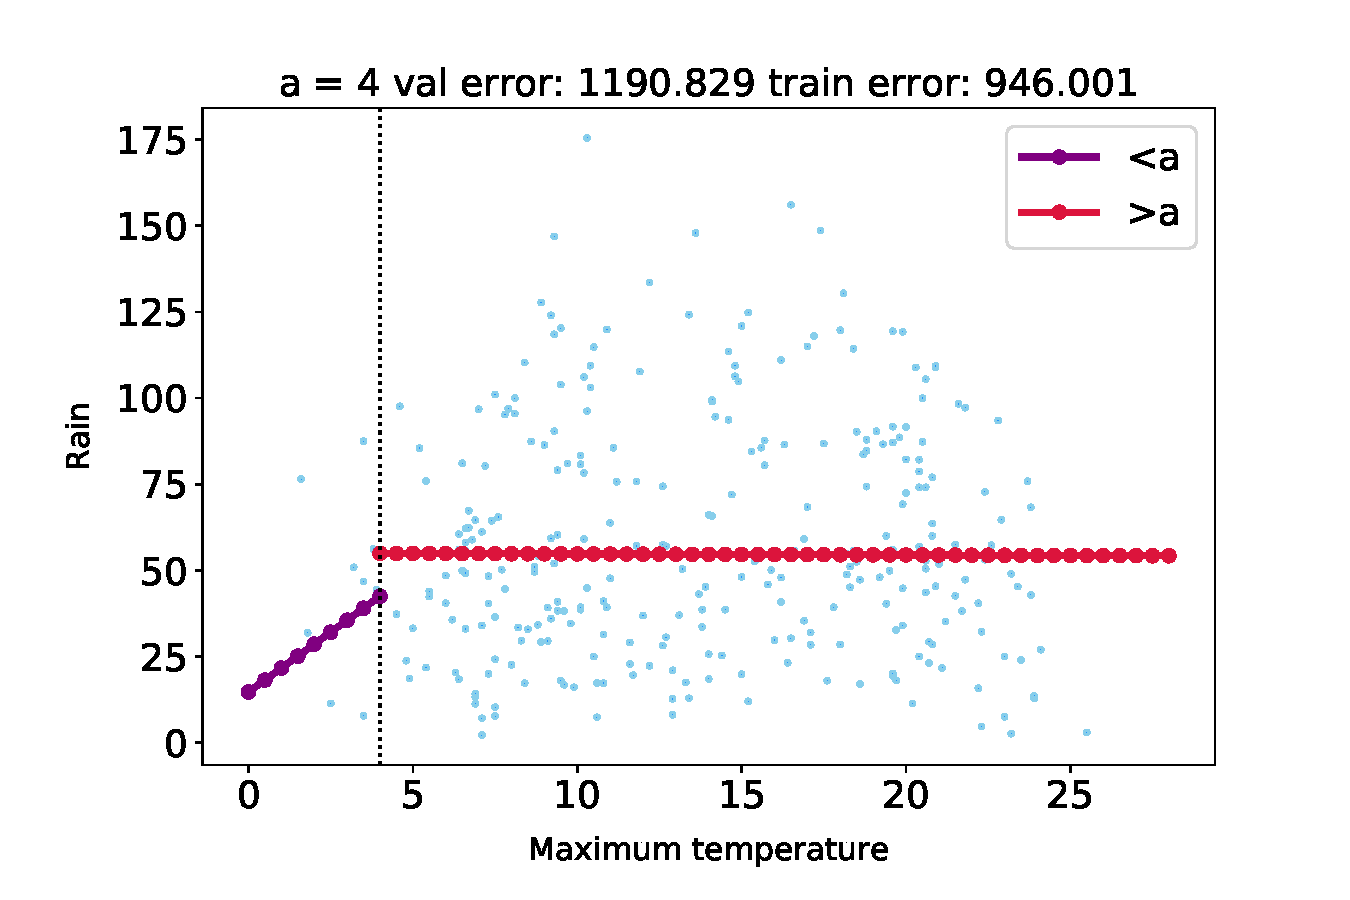
\includegraphics[width=200pt]{figures/a=4.pdf}
		\caption{Linear regression of rain fall as response of max. temperatures with $a=4$}
		\label{fig1}
	\end{figure}

	\begin{figure}[H]
		\centering
		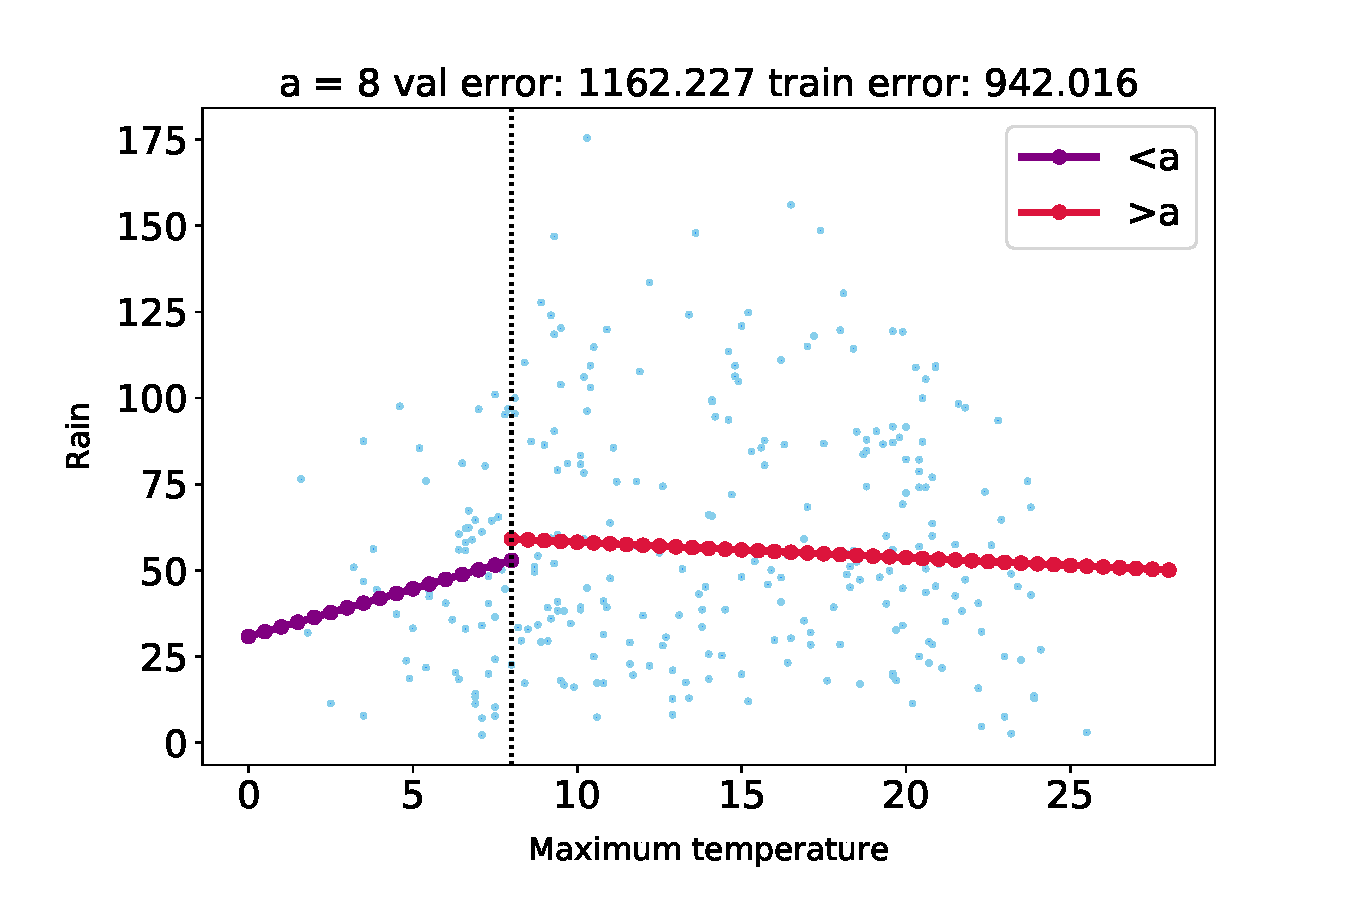
\includegraphics[width=200pt]{figures/a=8.pdf}
		\caption{Linear regression of rain fall as response of max. temperatures with $a=8$}
		\label{fig2}
	\end{figure}

	\begin{figure}[H]
		\centering
		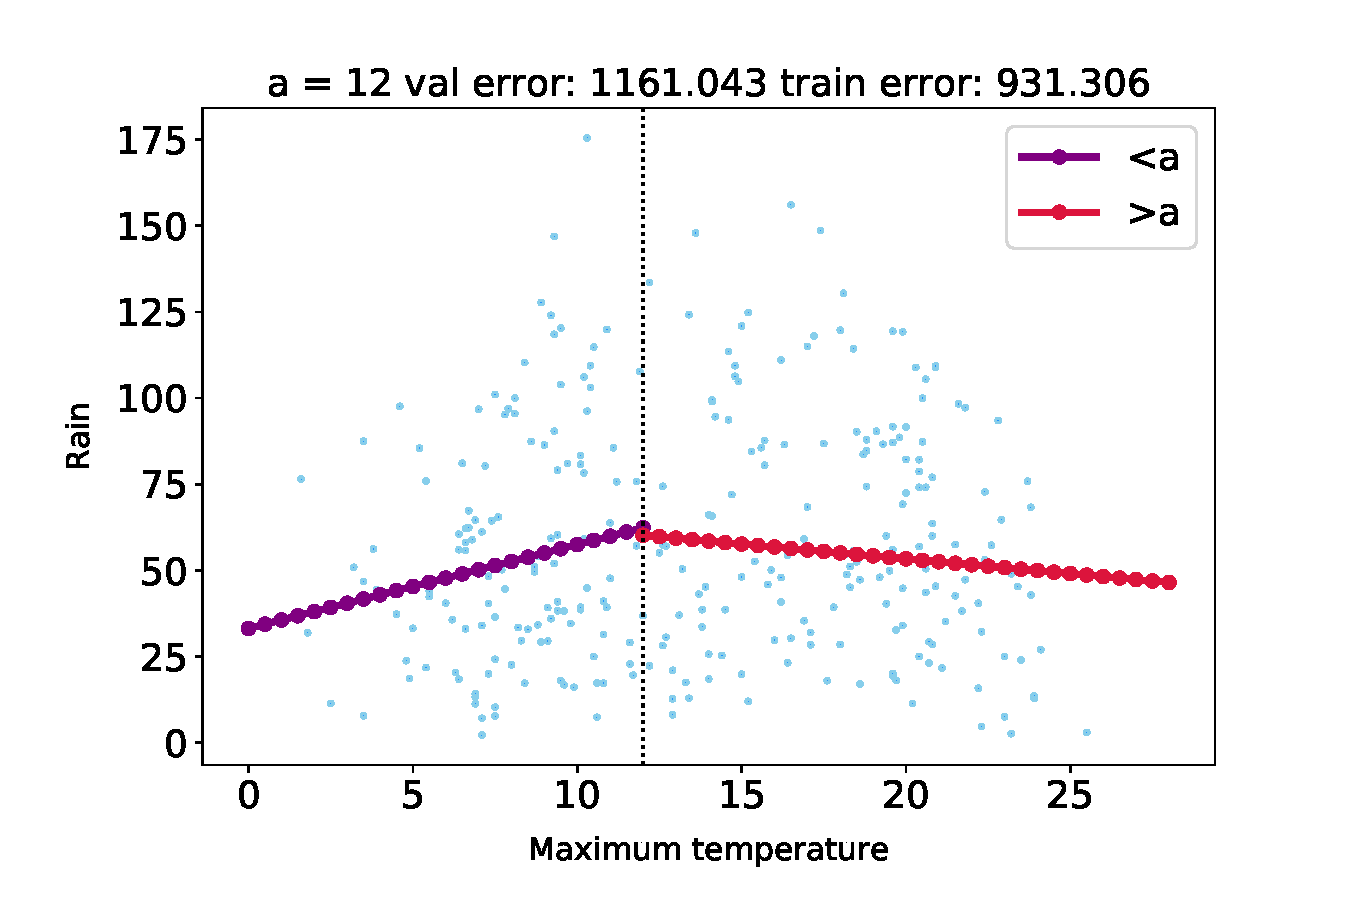
\includegraphics[width=200pt]{figures/a=12.pdf}
		\caption{Linear regression of rain fall as response of max. temperatures with $a=12$}
		\label{fig3}
	\end{figure}

	\begin{figure}[H]
		\centering
		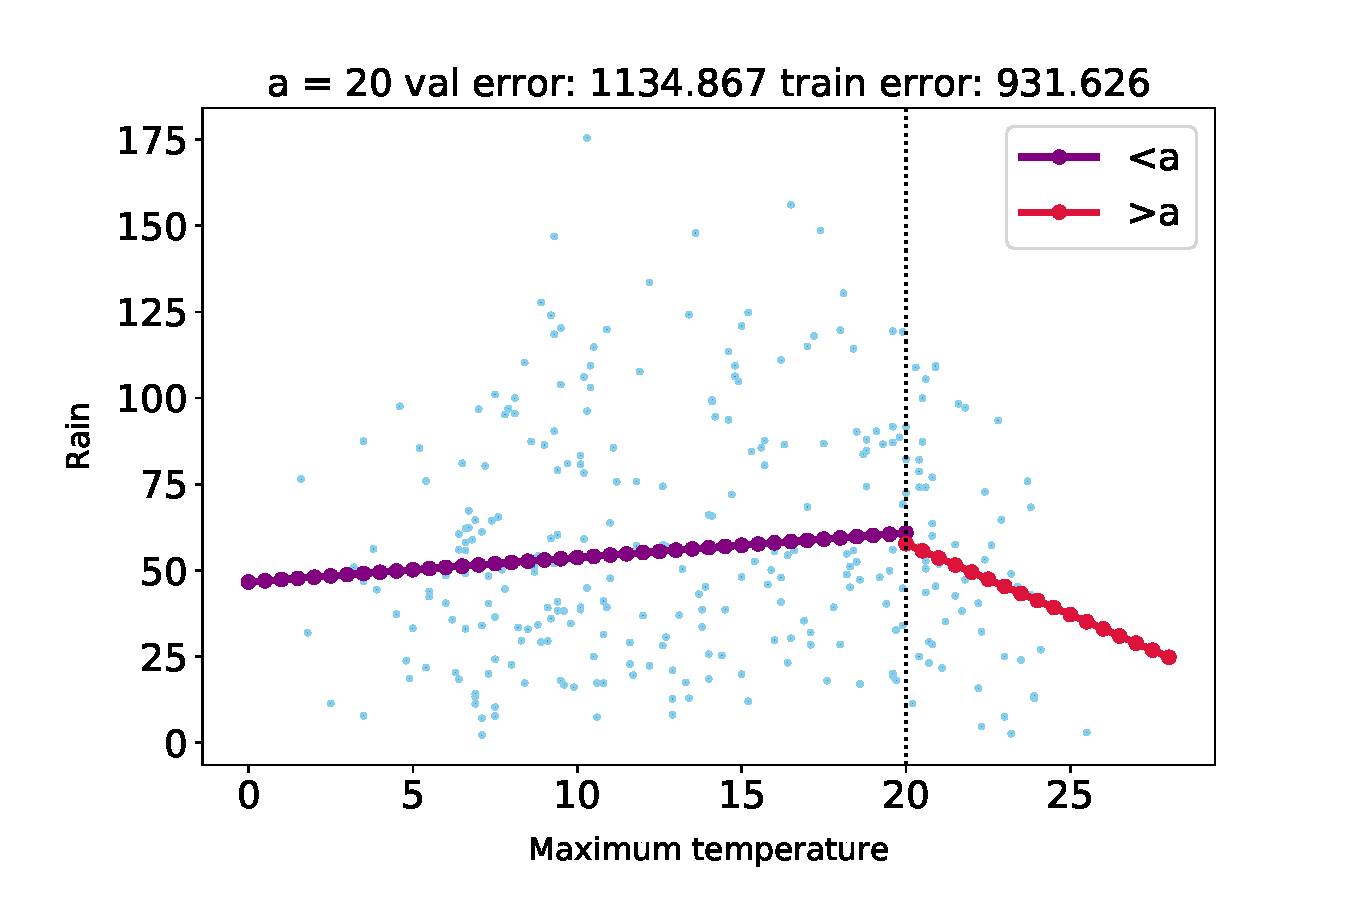
\includegraphics[width=200pt]{figures/a=20.pdf}
		\caption{Linear regression of rain fall as response of max. temperatures with $a=20$}
		\label{fig4}
	\end{figure}

	\begin{figure}[H]
		\centering
		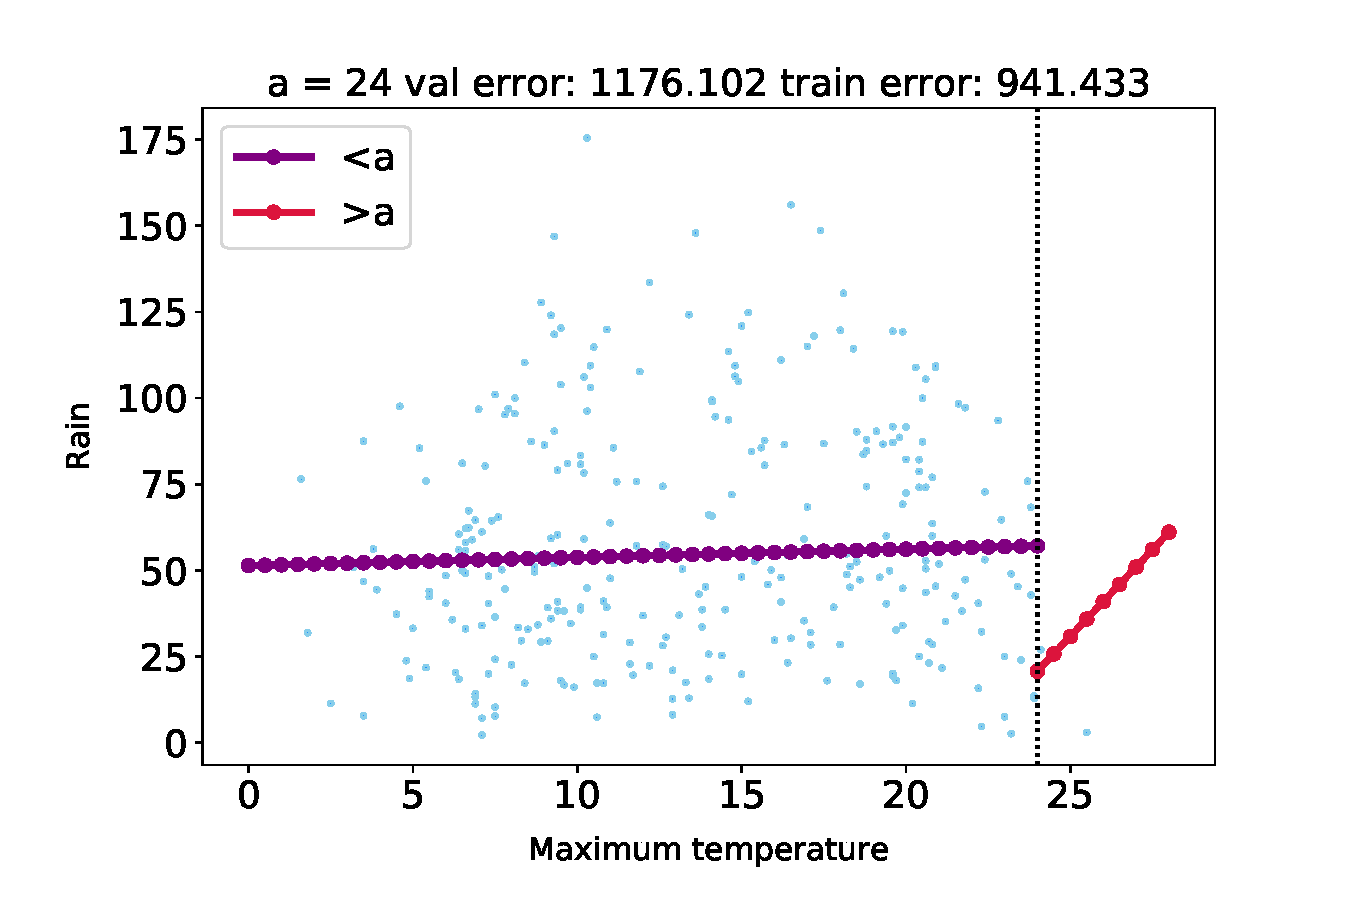
\includegraphics[width=200pt]{figures/a=24.pdf}
		\caption{Linear regression of rain fall as response of max. temperatures with $a=24$}
		\label{fig5}
	\end{figure}
	
 \item Choose the best estimator $f_{a'}(x)$ according to the validation error. Fill in the rest of \verb|main()| function to fit a single linear estimator on the entire dataset. Compare the fit and error values of $f_{a'}(x)$ with the single linear estimator fit on the training set on the held out test set.  Report the plot generated by this section. 
 
 	Having identified the best value $a$ to split the training data, we then train two linear models using this value of $a$ by splitting the entire training dataset between
	max.temperatures $\le a$ and max. temperatures $\ge a$ and fitting with the split on the rainfalls using the same value of $a$.
	We then train a linear model on the entire training set using the train maximum temperatures and train rainfall data.
	
 
 	\begin{figure}[H]
		\centering
		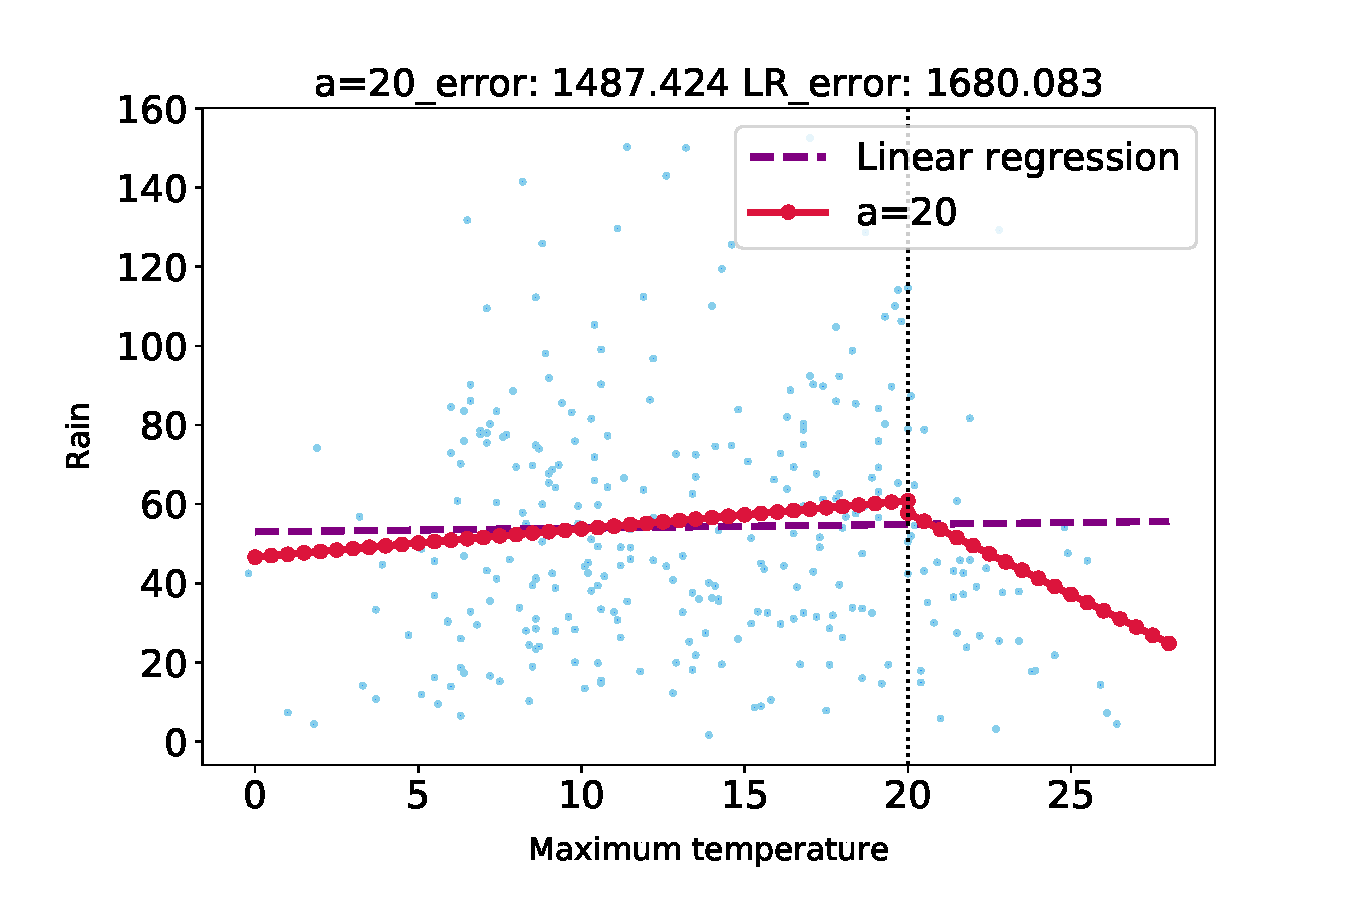
\includegraphics[width=200pt]{figures/test_comparison.pdf}
		\caption{Comparison between a single linear estimator fitted on the whole dataset and the  the best estimator $f_a'$}
		\label{fig6}
	\end{figure}


 \end{enumerate}
 	
 We do not require you to include your code in the report. You can choose to include it or not include it. 
\end{enumerate}
\end{document}
